\section{What trapped throughput does not tell}\label{sec:control}

\begin{figure*}[t]
\centering
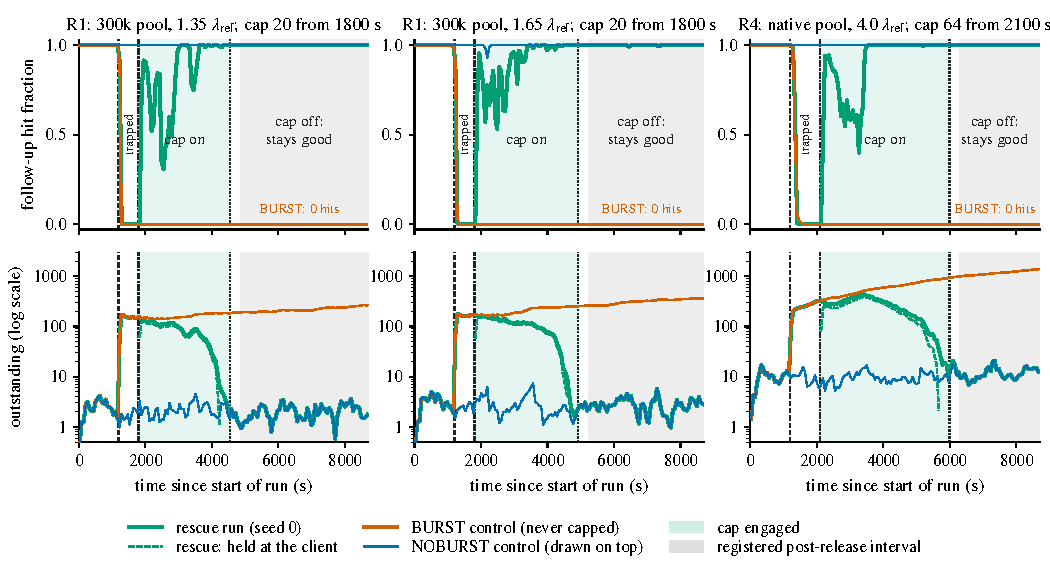
\includegraphics[width=\textwidth]{figs/fig_rescue.pdf}
\caption{Trap, rescue, release and persistence: the registered rescue tests R1 and R4, seed 0 of each cell. Each rescue run
(green) replays the arrival plan of a paired test's BURST run until a client-side session cap is engaged at $t_{\mathrm{on}}$
(dash-dotted); the cap is removed at
$t_{\mathrm{rel}}$ (dotted) once both client queues have been empty for 300\,s. The same-seed BURST (vermillion) and NOBURST (blue)
runs share its arrivals. Dashed: the burst of 200 sessions at 1200\,s. Top: follow-up hit fraction in 60\,s bins. Bottom:
outstanding work, requests in the engine plus sessions held at the client (log scale); dashed green: sessions held at the
client. Seeds 1 and 2 behave alike (Table~\ref{tab:rescue}).}\label{fig:rescue}
\end{figure*}

An operator who sees a trapped engine complete sessions at some rate may expect a cut to just below that rate to clear it.
Corollary~\ref{cor:trapthr} says that in model~F, for our workload, it does not: the trap clears only below $\lmiss$, after a busy period that diverges
as the cut approaches $\lmiss$. In the all-miss fluid at 1.65~$\lref$ (300k), a cut to $1.18\lmiss$, below $D=1.22\lmiss$, makes the
backlog dip by 0.3\% and grow again, and a cut to $0.9\lmiss$ drains it only after about 15 hours (Appendix~\ref{app:trap}). That
leaves two exits: starve the trap, which is slow and, done by refusing arrivals, sheds sessions; or leave model~F, by making turns hit
again, which needs the sessions that compete for the pool to fall below the all-miss onset $n_b$ (Appendix~\ref{app:entry}) without
lowering the offered load. Lu et al.\ reverse the outcome in simulation by lowering post-surge arrivals~\citep{lu2026cachetrap}; their
systems keep some reuse in the trap, so Corollary~\ref{cor:trapthr} does not describe them (Appendix~\ref{app:lu}).

\paragraph{Cutting arrivals: CUT-A and CUT-B (blind in outcome).} CUT tests the corollary's setting on the engine: the 1.65~$\lref$ BURST
protocol, then from 2400\,s arrivals cut to 1.15~$\lref$ (CUT-A, $\rho'=1.145$, inside $(\lmiss,D(\lambda))$) or to 0.85~$\lref$
(CUT-B, $\rho'=0.846$), seeds 0--2. Model~F's predictions, driven by each seed's exact client plan, were frozen under tag
\texttt{icml-cut-pred}: all six runs stay stuck over $[5700,8700)$\,s; CUT-A, although its rate is below the trapped throughput of
the same seed's uncut run, does not clear, its backlog dipping by less than 15\% on 300\,s bins and growing again in seeds 0 and 2 (seed~1's plan
has few post-cut arrivals); CUT-B's backlog shrinks slowly and would empty only at about 27{,}100\,s, the busy period of
Proposition~\ref{prop:classic}(a). The decision rule, registered after the predictions were pushed and before any CUT job (tag
\texttt{r15-cut-reg}), compares each seed's backlog slope $S$ over $[3000,8700)$\,s with model~F's frozen slope and with two
constant-throughput comparators: a naive one, in which the trap drains at the trapped throughput of the same seed's uncut control
(1.32--1.41~$\lref$), and, for CUT-A, a quasi-static one, in which it completes sessions at $\lref$. A seed is theory-favoured if
model~F's slope is strictly the closest; an arm passes if at least 2 of 3 seeds are theory-favoured and a sign clause holds, and fails if a
comparator is favoured, or the run leaves the trap, in 2 of 3. The rule was fixed after the per-seed predictions had been read, and it
differs from the draft rule simulated in the prediction note in five ways: three stricter, one stricter for two seeds and looser for
the third, and one looser, which in the note's simulation raised CUT-A's probability of passing from 0.82 to 0.99
(Appendix~\ref{app:blind}).

Both arms passed. With arrivals cut to a realized 1.12--1.20~$\lref$, all three CUT-A runs stayed stuck to the end at zero hits, and
all three seeds were theory-favoured: slopes of $+0.0040$, $-0.0022$ and $+0.0029$\,/s against model~F's $+0.0039$, $-0.0026$ and
$+0.0028$, the naive comparator's $-0.0094$ to $-0.0204$ and the quasi-static one's $+0.0086$ to $+0.0146$. After the cut to a realized
0.81--0.88~$\lref$, the CUT-B backlog fell, slowly, at $-0.0085$ to $-0.0126$\,/s against model~F's $-0.0095$ to $-0.0131$ and the
naive $-0.033$ to $-0.043$; all three seeds were theory-favoured, and all three runs were still stuck at 8700\,s, with 140, 77 and 89
sessions present against model~F's 139, 79 and 94.

The passes are narrower than the corollary. Both comparators assume a constant throughput, so each rule rejects only the
constant-throughput readings it was built against: the naive one in both arms and, in CUT-A, the quasi-static one. Intermediate
readings fit as well: over $[3000,8700)$\,s constant completions at the nominal cut rate fit CUT-A as well as model~F, and the
quasi-static reading, not a registered comparator for CUT-B, fits its slopes about as well (had it been one, CUT-B would still have
passed, 2 of 3). What singles out model~F against them is post hoc: CUT-A's late-window slopes ($+0.0071$, $-0.0027$ and $+0.0131$\,/s
against model~F's frozen $+0.0069$, $-0.0036$ and $+0.0129$, while constant completions at the trapped throughput, at $\lref$, at their
midpoint or at the nominal cut rate each missed by about 0.004\,/s or more) and CUT-B's completions below the all-miss capacity as the trapped mix aged (0.918--0.974~$\lref$ against model~F's
0.918--0.979, although at the frozen tolerance the all-miss capacity also lies just inside). Persistence discriminates only in part:
every constant reading also leaves CUT-A stuck to 8700\,s, so there it rules out only a drain at the completion rate seen just before
the cut (1.21--1.70~$\lref$ over $[1800,2400)$\,s), which would have reached the onset near 6300\,s in seeds 0 and~1, the operator-facing
content of Corollary~\ref{cor:trapthr}; in CUT-B the naive reading, or a drain at the pre-cut completion rate, would have reached the
onset by 4900--7600\,s. The test has limits: the cut comes 1200\,s after the burst, so it probes the young trap's transient and the start
of its regrowth, not the asymptotic rate; CUT-B cannot show recovery within the run; CUT-A's runs shared one node and CUT-B's ran on
two; and ``did not clear'' means within 8700\,s.

\paragraph{Refusing arrivals sheds sessions (SHED).} The registered SHED test at 1.35~$\lref$ on the 300k pool stopped arrivals
entirely from 1800\,s, 600\,s after a burst. A 600\,s stop refused 56--59 sessions and left both runs stuck; a 3600\,s stop refused
355--378 and left both good, hits returning 2300--2600\,s into the stop (post hoc). In model~F the fluid backlog falls to the onset $n_b=32.7$
after 2{,}020\,s of the stop and the queue empties after 3{,}180\,s, the remaining work $V_{\mathrm{tot}}(1800)$
(Proposition~\ref{prop:classic}(a)); the quasi-static model's frozen minimum stop was 1{,}795\,s, early by about a quarter, and
model~F's time to the onset is early too, by about 15\%. Model~F's numbers are a retrodiction, computed after the SHED runs had ended,
and the test does not discriminate: any drain time between 600 and 3600\,s fits its two stop lengths.

\paragraph{Restoring reuse with a session cap.} A FIFO gate that admits at most $\ncap$ sessions, each holding its slot until its
last turn ends, makes the admitted sessions a closed system of $\min(n,\ncap)$ sessions (Proposition~\ref{prop:cap}, Appendix~\ref{app:qs}). In the
quasi-static model the gate then empties if and only if $n_1<\ncap<n_2$, the stable and unstable fixed points of
$\dot n=\lambda-\mu(n)$, and once it is empty and removed the population stays in the good state's basin
(Corollary~\ref{cor:rescue}, Appendix~\ref{app:qs}). In model-F terms the cap keeps the admitted sessions below the onset, so their turns hit again, and the
excess waits at the client instead of in the engine's queue, where every turn would miss. The registered rescue tests R1 (300k pool,
cap 20, engaged at 1800\,s, 600\,s after the burst, at 1.35 and 1.65~$\lref$) and R4 (native pool, cap 64, at 2100\,s, at
4.0~$\lref$) engaged the registered CAPPED caps inside established traps: follow-up hit fraction 0.000--0.002 over the preceding
300\,s, with 139--324 requests or sessions outstanding. All 9 runs were rescued without shedding a session (Fig.~\ref{fig:rescue};
Table~\ref{tab:rescue}). Hits returned within three minutes, the backlog drained, and the cap was released at 3980--6140\,s, once the
client queues had been empty for 300\,s. With the cap removed, every run stayed good at the same arrival process for the remaining
2560--4720\,s, matching its NOBURST control in follow-up hit fraction, outstanding work and turn latency, while the same-seed uncapped
BURST run stayed at zero hits. The price is waiting at the client: 386--569\,s per paused session on average, 38--78 (300k) and 222--230
(native) session-hours per run. In a slowdown-only form of Lu et al.'s SLO goodput (their
inter-token-latency condition omitted, our own unloaded reference; post hoc, Appendix~\ref{app:dataonly}), the burst cost all 30
registered BURST runs 99.2--100\% of the next hour's goodput against the same-seed NOBURST run, and the rescue 45--97\% (depending
on the reference), but the rescue restored the evaluation window's goodput to within 1\% of NOBURST.

\paragraph{What the rescue does and does not show.} Persistence here means that the drained state sustains itself once the cap no
longer binds: the release rule waits until the gate is empty, so the tests do not cover a release while the cap still binds, and
the cap is engaged at a fixed time, not on an online signal. The frozen first-principles model predicted the rescue in every cell,
but 4 of its 9 release times fell outside its $\pm15$\% tolerance (R4 released 19--22\% late; Appendix~\ref{app:rescuetests} and Table~\ref{tab:frozensum}). Lu et
al.\ restore service on hardware by terminating the burst sessions at the end of the burst, when the trap is incipient, prevent it
with their controller active before the surge, and rescue an established trap in simulation by activating their controller late
(and leaving it armed: its admission releases itself after a cool-down, but no reported run removes the controller and tests
persistence; Appendix~\ref{app:lu}). What our tests add is a registered, replicated rescue of an \emph{established} zero-hit trap on
the engine at the same offered load, without shedding, with the control removed and the good state persisting after it.
